\chapter{Forschungsplan}

Folgend wird beschrieben zu welchem Zeitpunkt mit welchen Methoden die Messwerte erhoben werden um im Anschluss die zwei Technologien miteinander vergleichen.

Um die zwei verschiedenen Technologien zu vergleichen sollen zwei Testnetzwerke aufgebaut werden.
Jeweils eines pro Technologie.
Diese Netzwerke werden genutzt um sie hinsichtlich ihrer verschiedenen Eigenschaften zu testen.
Jedes Netzwerk wird dabei zwei Nachbargebäude der Hochschule verbinden um als Prototyp für ein größeres Netzwerk dienen zu können.
Zur Vergleichbarkeit werden für beide Netzwerke die selben Endpunkte definiert.

\section{Inbetriebnahme}\label{inbetriebnahme}

Ein Teil des Forschungsaufwandes wird dabei schon während des Baus und der Inbetriebnahme geleistet.
Dabei werden verschiedene Phasen unterschieden.

\begin{description}
    \item [Planung des Standorts der Endpunkte]\hfill \\
        In dieser Phase werden die Standorte der zwei Endpunkte, welche von beiden Netzwerken genutzt werden, geplant.
    \item [Planung des Transportwegs]\hfill \\
        Die Planung des Transportwegs umfasst den Weg der Datenleitungen und die Standorte von benötigter Hardware.
    \item [Installation der Kommunikationshardware]\hfill \\
        In dieser Phase wird die Leitung und benötigte Hardware aufgestellt.
    \item [Installation der Endpunkte]\hfill \\
        Diese Phase beinhaltet die Installation von den Computern und der Hardware, welche benötigt wird weitere Tests durchzuführen.
    \item [Einrichten der Netzwerke] \hfill \\
        Nachdem die Hardware bereit ist, muss die Software zum Betreiben der Netzwerke eingerichtet werden. Dies geschieht in dieser Phase.
    \item [Abschließende Funktionstests] \hfill \\
        Die Abschließenden Funktionstests haben die Aufgabe Probleme im weiteren Verlauf zu vermeiden.
        In dieser Phase kann es zu Nacharbeiten kommen, welche die Phase verlängern.
\end{description}

Für jeden der Schritte werden mehrere Vergleichsgrößen dokumentiert und anschließend gewichtet gewertet.

\begin{itemize}
    \item Anzahl der nötigen Kommunikationspartner
    \item Personenstunden
    \item Personalkosten
    \item Materialkosten
    \item Benötigte Zeit des Arbeitspakets
    \item Ergebnisse des Funktionstests
\end{itemize}

\section{Experimente}

Im Anschluss an den Bau und der Inbetriebnahme werden Experimente durchgeführt.
In der einjährigen Phase der Experimente werden Kenngrößen wie Datendurchsatz, Zuverlässigkeit und Energiebedarf ermittelt.
Zusätzlich soll die Sicherheit mit mehreren Experimenten untersucht werden.

Der Datendurchsatz wird mittels einem eigenen Skript getestet.
Dieses nutzt eine \ac{TCP} Verbindung um mehrere definierte Pakete vom Sender zum Empfänger und zurück zum Sender zu verschicken.
Durch die \ac{TCP} Verbindung wird sichergestellt, dass die Nettodatenrate gemessen wird, welche für eine Einschätzung der Geschwindigkeit während einer Vollständige Kommunikation relevant ist.
Dieses Skript wird regelmäßig ausgeführt um eine Entwicklung über die gesamte Phase hinweg zu dokumentieren.

Um die Zuverlässigkeit vergleichen zu können werden alle nötigen Wartungsarbeiten und Ausfälle sowie Aufwände für diese Dokumentiert.
Diese werden zusammen mit den Kosten und Aufwänden der Inbetriebnahme betrachtet und gewertet.

Während der gesamten Zeit wird der Energiebedarf aller Komponenten gemessen und zusammen mit der aktuellen Last des Netzwerkes.
Allerdings wird der Energiebedarf nicht dem eines Netzwerkes im operativen Einsatz entsprechen.
Allerdings ist es durch die Betrachtung des Energiebedarf abhängig von der Last möglich den Energiebedarf für operative Netzwerke zuverlässig zu schätzen.

Der größte Aufwand in der Experiment Phase werden die Experimente zur Sicherheit der Netzwerke beanspruchen.
In den Experimenten werden bekannte Sicherheitslücken der jeweiligen Technologie verwendet um an den Schlüssel zu gelangen.
Während der Durchführung der Experimenten werden, genauso wie bei der Inbetriebnahme, alle Kosten, Aufwände und die Dauer dokumentiert.
Im Fall von einer Beschädigung der Hardware durch die Experimente, werden die anfallenden Kosten für die Reparatur nicht in die Wartungskosten des Netzwerkes eingerechnet.
Der Vergleich der Netzwerke in Bezug auf die Sicherheit erfolgt anhand des Erfolgs der Angriffe, genauso wie den erhobenen Daten während der Durchführung des Angriffes.

\section{Auswertung}

Nach einem Jahr werden alle Ergebnisse gesammelt und ausgewertet.
Die in Kapitel~\ref{forschungsstand} bereits beschriebenen Eigenschaften zeigen, dass die zwei Technologien sehr verschieden sind.
In der Auswertung werden die in Sektion~\ref{inbetriebnahme} beschriebenen Eigenschaften zusammen mit den Betriebskosten und den Ergebnissen der Experimente gegenübergestellt.
Trotz der großen Unterschiede werden die einzelnen Eigenschaften gewichtet um am Ende eine Empfehlung für die Hochschule München aussprechen zu können.

\section{Zeitplan und Resourcenplan}

Aus den vorherig beschriebenen Punkten ergeben sich insgesammt zehn Arbeitspakete und drei Meilensteine während des Projekts.
Für jedes Arbeitspaket ist eine Anzahl an Personen geplant, die mit dem jeweiligen Arbeitspaket befasst sind.
Das Ergebniss aus dieser Planung ist folgendes Gantt-Chart.

\begin{figure}[htbp] 
  \centering
     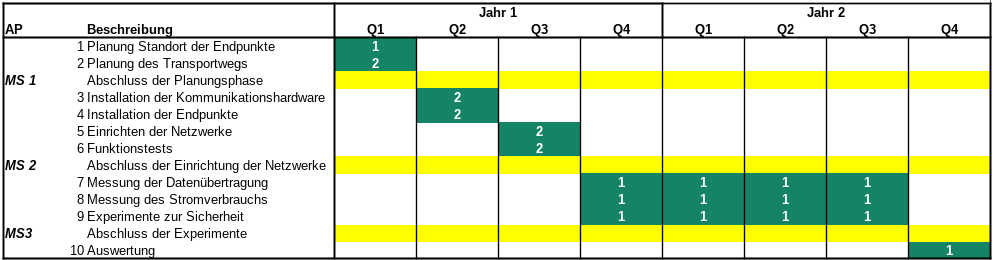
\includegraphics[width=1\textwidth]{img/gannt.png}
     \caption{Gantt-Chart zum Projekt mit den Arbeitspaketen in Grün, den Meilensteinen in Gelb und der Anzahl an benötigten Personen in Weiß innerhalb der Arbeitspakete.}
     \label{fig:gantt}
\end{figure}

Damit ist das Projekt nach zwei Jahren abgeschlossen.

